\documentclass[a4paper]{article}
\usepackage[margin=1in]{geometry}


%%%%lualatex on
%\usepackage{luatextra}
%\usepackage{fontspec}
%%Ligatures={Contextual, Common, Historical, Rare, Discretionary}
%\setmainfont[Mapping=tex-text]{Linux Libertine O}
%%Phd Description after meeting with Xavi on the 27th of July

\usepackage{natbib}
\usepackage{graphicx}


\title{Research Plan}
\author{Simon Carrignon}

\begin{document}

\vspace{-1cm}
\hspace{-1cm}
\begin{minipage}{.5\textwidth}
	\noindent \includegraphics[width=5cm]{images/upfLogo.jpeg} 
\end{minipage}
\hfill
\begin{minipage}{.5\textwidth}
    \flushright
	\textbf{ \Large RESEARCH PLAN }
\end{minipage}

	\vspace{3cm}

{

\noindent\textbf{Student:} Simon Carrignon
\vspace{.5cm}

\noindent\textbf{Project Title:} ``Cultural evolution and long term economic dynamics: The case study of Rome.''
\vspace{.5cm}

\noindent\textbf{PhD thesis supervisors:} Xavier Rubio-Campillo \& Sergi Vavlerde
\vspace{.5cm}

\noindent\textbf{Research Group:} Barcelona Supercomputing \& Center Complex System Lab (UPF)  
\vspace{.5cm}

}
\vspace{2cm}

\noindent\textbf{\LARGE Research Plan: }


%\section{Introduction}
%    \begin{description}
%	\item[School:] UPF PhD Programme in Biomedicine 
%	\item[Supervision:] Xavier Rubio (BSC) \\ Sergi Valverde (UPF-Complex System Lab)
%	\item[Funding:] 4-years grant from EPNet project \\ (ERC advanced Grant 340828):
%    \end{description}
%
%    \begin{quote}
%	\small
%	Production and Distribution of Food during the Roman Empire: Economic and Political Dynamics
%    \end{quote}
%    \vfill
\section*{Introduction}
\subsection*{Cultural Evolution}
In this thesis we are interested to how social traits evolve. By social traits we mean every thing that have been culturally transmitted and or socially learnt. Thos traits often exhibits similar patterns of adoption and evolution and are widely studied by people that are studying Cultural Evolution. 

The aims of this fields of research is to understand:\\

\begin{minipage}{\textwidth}
    $\rightarrow$ What mechanism drive the evolution of such traits?\\
    $\rightarrow$ What mechanism generate such pattern?
\end{minipage}
\vspace{2cm}

Research have shown that simple mechanisms (Bentley et al, 2004) can model such pattern such as Random Copy , Frequency biased (conformist/anti-conformist\dots) and other.

\begin{figure}
    \centering
    \includegraphics[width=10cm]{images/powerlawrepartition.jpg}
    \caption{Square: male names,Circle: female names, Dotted and plain lines: model result with different copy probabilities.From Bentley et al,~2004.}

\end{figure}
\subsection*{Co-Evolution of Culture and Trade}
More precisly, what happen when those social traits are linked to economical activities

%	    \only<2>{\vspace{1cm}\includegraphics[height=3cm]{images/bordeaux.jpg}\hspace{2cm}
%	    \includegraphics[height=3cm]{images/napa}}
%	    \only<3>{\includegraphics[height=4cm]{images/tools}}
%	    \only<4>{\includegraphics[height=4cm]{images/stockoption}}
\begin{figure}
    \centering
    \includegraphics[width=10cm]{images/interaction}	
\end{figure}
%
%\end{frame}
%
%
%
\subsection*{Approach}


\begin{itemize}
    \item Archaeology
	\begin{itemize}
	    \item Compare culture across time (vs ``twitter studies'')
	\end{itemize}
	\vfill
    \item Computer Simulation
	\begin{itemize}
	    \item Compare \& Select models
	    \item Explore \& Generate hypothesis
	\end{itemize}
\end{itemize}
%
\begin{figure}
    \includegraphics[width=2cm]{images/approach.pdf}		
\end{figure}
%    
%\end{frame}
%
%\begin{frame}
%    \begin{center}
%	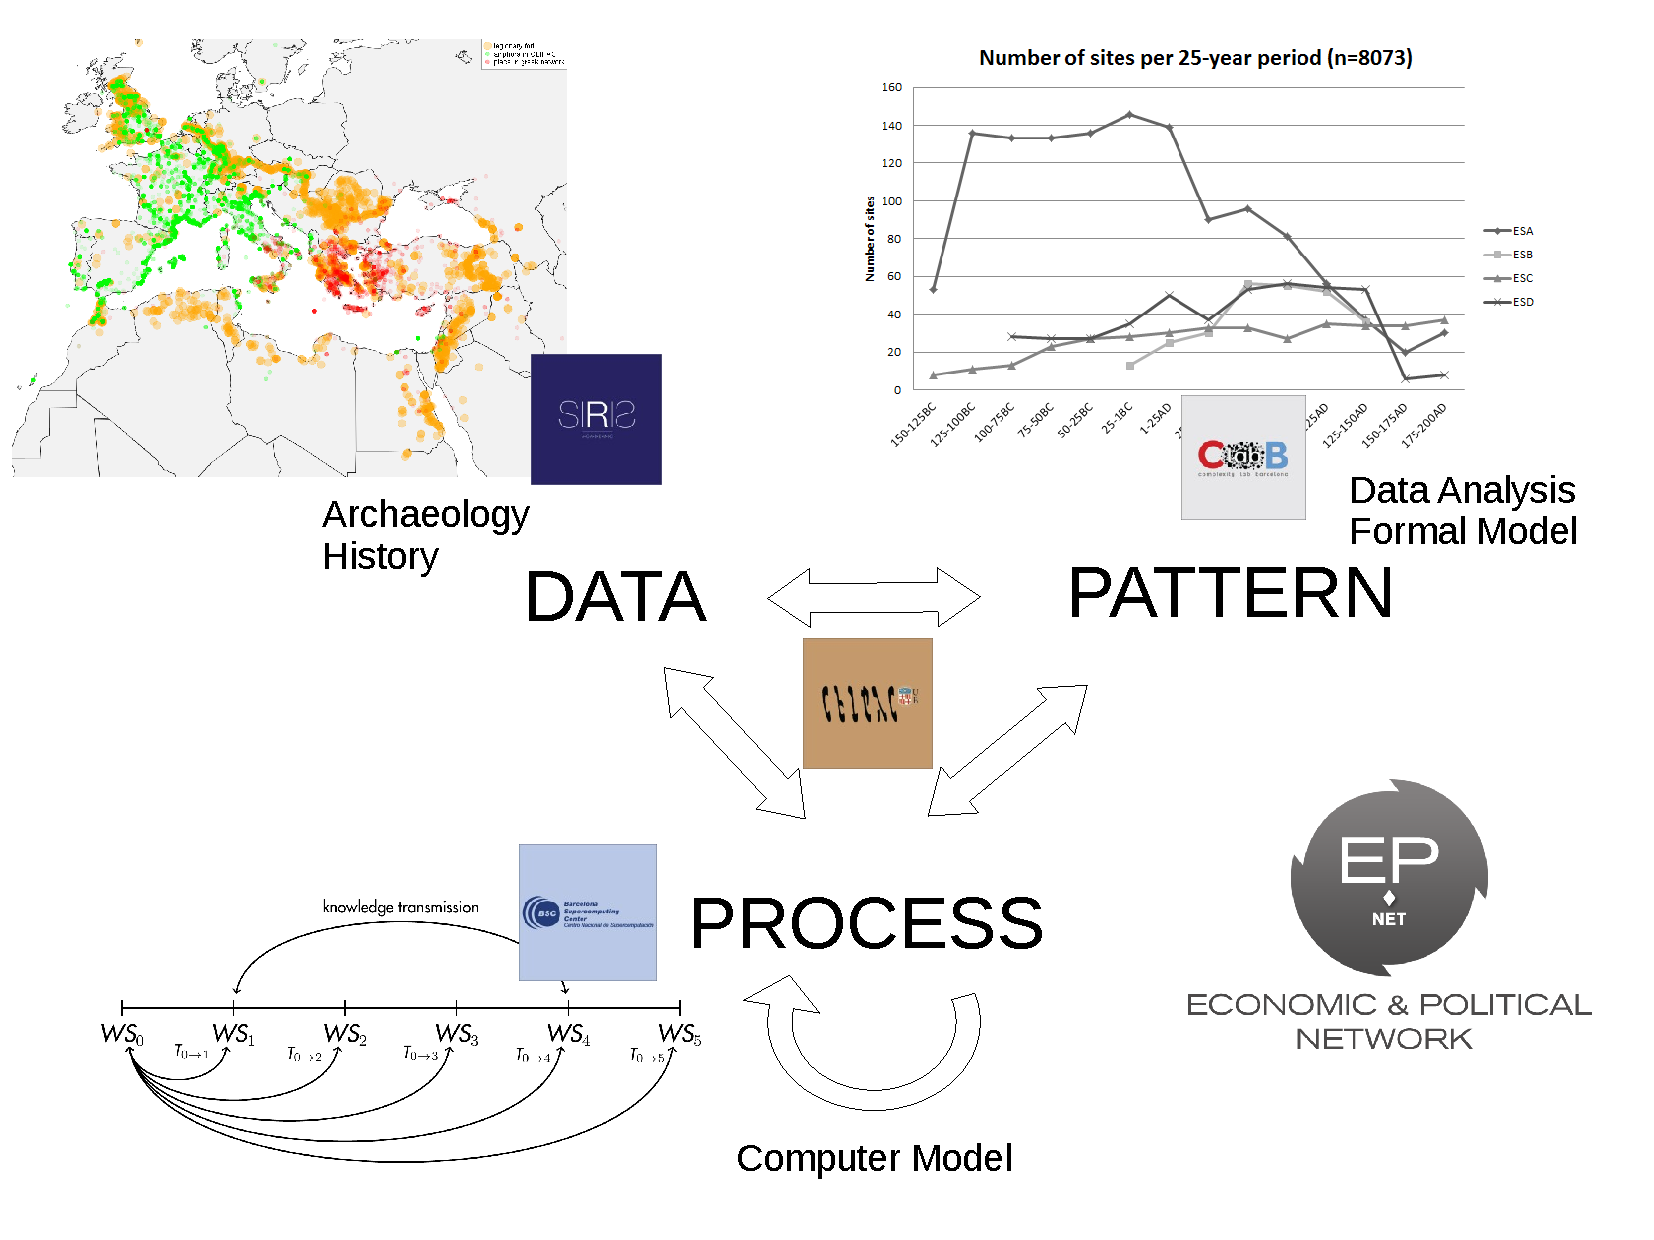
\includegraphics[width=\textwidth]{images/approach2.pdf}		
%    \end{center}
%    
%\end{frame}
%
%\begin{frame}
%    \centering
%    \Large
%   Plan 
%\end{frame}
%\begin{frame}{Plan}

\section{Theoretical Exploration: How economics value change the dynamics of Cultural Evolution (Computer Model vs Neutral Model) }
\section{ Empirical Study:  Characterize an economy through socio-economic artefacts distribution, a case study the Roman Empire (Scaling Properties)}
\section{ Articulate the Theoretical Exploration \& the Empirical Observations}
%
%\end{frame}
%
%\begin{frame}
%    \centering
%    \Large
%    Theoretical Exploration
%\end{frame}
%
%\begin{frame}{A General Agent Based Framework }
%
%     Two main components:
%     \vfill
%    \begin{enumerate}
%	\item Trade side: Bartering Economy (Gintis 2009),
%	\item Cultural side: ``copy the most successful'' (Bentley 2006).
%    \end{enumerate}
%    \begin{center}
%	\includegraphics[width=.8\textwidth]{images/interaction}	
%    \end{center}
%\end{frame}
%	
%
%\begin{frame}{The Model}
%	\begin{block}{1. The Economy \& the Barter Mechanism}
%		\begin{itemize}
%			\item $N$ goods
%			\item $M$ Agent 
%				$\left\{
%					\begin{tabular}{@{}l@{}}
%						a quantity of each Goods \\
%						$N$ values attributed to each goods\\
%					\end{tabular}
%					\right.$
%				\item Agents \emph{produce} one good and \emph{exchange} it to obtain the other goods.
%				\item After the exchange, the agents \emph{consume} all goods 
%			\end{itemize}
%			Agent perform this 10 times and a scores is given to each of them.
%		\end{block}
%	\end{frame}
%
%	\begin{frame}{The Model}
%		\begin{block}{2. Cultural Mechanisms}
%			\begin{itemize}
%					\vfill
%				\item Less successful agents \emph{copy} the most successful (Biased-Copy).
%					\vfill
%				\item Given a probability $\mu$ the value attributed to some goods is modified (Innovation/Mutation)
%			\end{itemize}
%		\end{block}
%	\end{frame}
%\begin{frame}{Experiments}
%	\centering
%	\textbf{Trade Model} \\Trade Mechanism + Success Biased Copy\\
%	\vfill
%	vs\\
%	\vfill
%	\textbf{Neutral Model}\\ Trade Mechanism + Random Copy\\
%	 
%
%\end{frame}
%
%
%\section{Results}
%
%
%
%\begin{frame}{Results: Economic Dynamic}
%    \begin{figure}[!h]
%	\centering
%	\begin{tabular}{ c c}
%	    Neutral Model & Trading Model \\
%	    \includegraphics[width=5cm]{images/ScoreEvolutionForRandom-G3N500.pdf}
%	    & 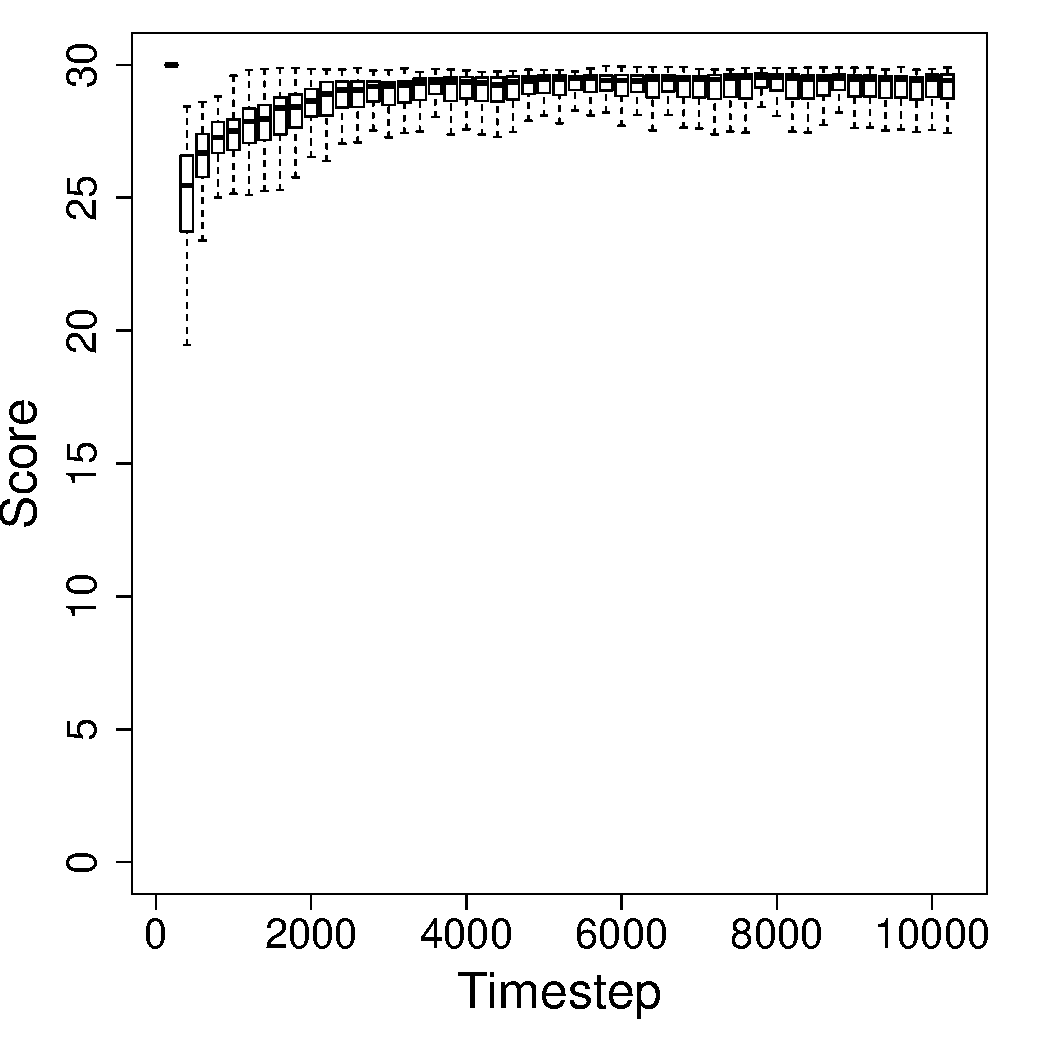
\includegraphics[width=5cm]{images/ScoreEvolutionForTrade-G3N500.pdf}
%
%	\end{tabular}
%	\caption{Evolution of the score within the two different models for two typical run with 500 agents and 3 goods evolving during 10000 timestep.}%%
%	\label{fig:scoreEvol}
%    \end{figure}
%\end{frame}
%    
%
%
%\begin{frame}{Results: Economic Dynamics}
%	\begin{figure}
%	    \caption{Example for 3 goods and 500 agents}
%	    \begin{columns}
%		\column{.5\textwidth}
%		\includegraphics[height=\textwidth]{images/ClearingPriceDistanceEvolutionForTrade-G3N500.pdf}\\
%	    \end{columns}
%		@~Equilibrium: personal values  $\rightarrow$ optimal (shared) values.
%	\end{figure}
%	
%\end{frame}
%
%\begin{frame}{Results: Frequency Distribution}
%    \subsection*{Distribution of variant:}
%    \begin{figure}[!h]
%	\begin{center}
%	    \begin{tabular}{ccc}
%		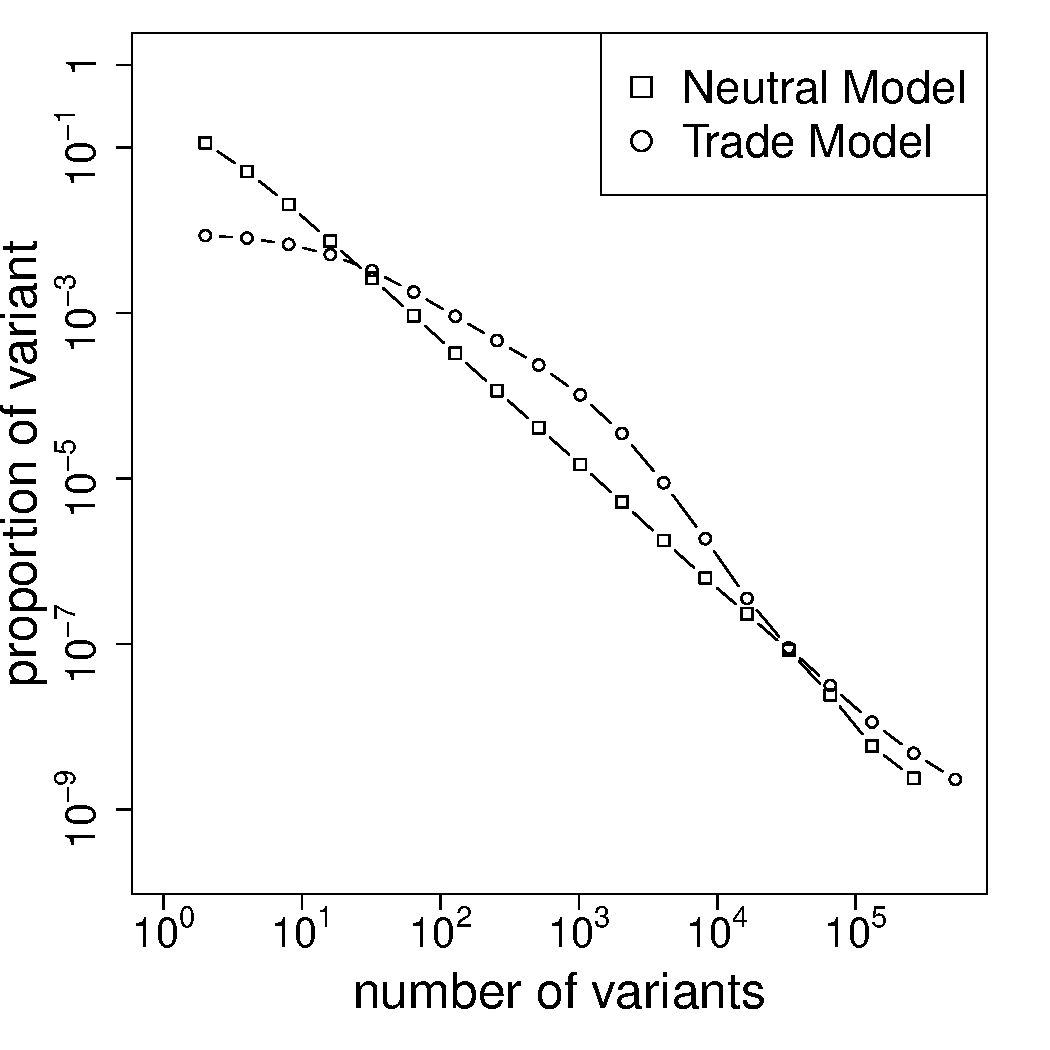
\includegraphics[width=5cm]{images/2SetupDistribA.pdf}\\
%	    \end{tabular}
%
%	\end{center}
%	%\caption{Frequencies distribution, where each points represent the mean for 100 runs, for: a) the neutral and the trading models.  b) the neutral model and the trading model without the trading innovation process. c) the trade model and the trade model without the trading innovation process.}
%    \end{figure}
%\end{frame}
%
%\begin{frame}{Next Objectives}
%    \vfill
%    Understand general dynamics and properties of such systems:
%    \vfill
%	\begin{itemize}
%	\item Parameters fitting
%    \vfill
%	\item Different Cultural Mechanisms
%    \vfill
%	\item Different Trade Assumption
%    \vfill
%	\item Network Constraints
%    \vfill
%	\item \dots
%    \vfill
%	\end{itemize}
%\end{frame}
%
%\begin{frame}
%    \centering
%    \Large
%   Empirical Studies 
%\end{frame}
%\begin{frame}{Empirical Studies}
%	Characterize an economy through socio-economic artefacts distribution:\\
%	\hspace{1cm} The need of strong proxy\\
%
%	\vspace{.5cm}
%    \uncover<2->{
%	    Within EPNet:
%	    
%    \begin{itemize}
%	\item Olive Oil production
%	\item Wine production
%	\item \ldots
%    \end{itemize}}
%    \uncover<3->{
%	    \begin{alertblock}{Intuition}
%		    Scaling properties of those indicators across cities to infer economic properties
%	    \end{alertblock}
%    }
%\end{frame}
%
%\begin{frame}{Scaling properties}
%    \begin{figure}
%	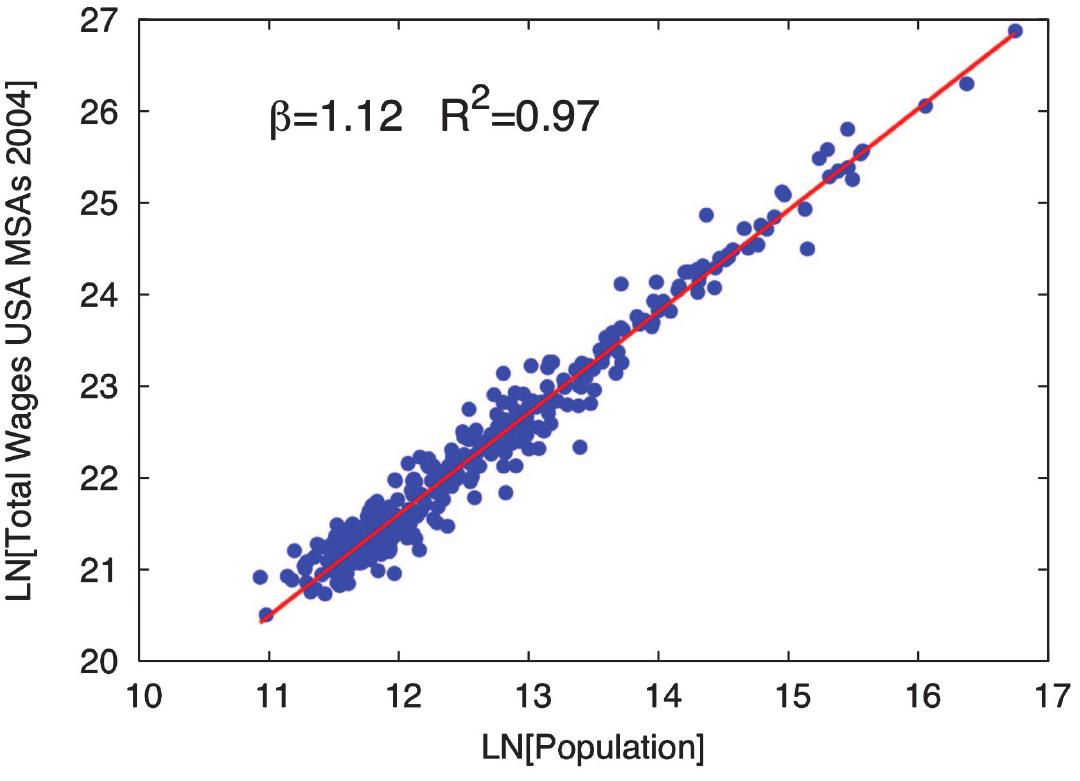
\includegraphics[width=.8\textwidth]{images/wageVsSize.jpg}
%	\caption{ Bettencourt 2007}
%    \end{figure}
%\end{frame}
%
%
%
%\begin{frame}
%    \centering
%    \Large
%    \section{  Last Part}
%\end{frame}
%
%\begin{frame}
% To what extent the theoretical model can explain the observed patterns?
%    
%
%\end{frame}
%
%\begin{frame}{So far}
%    \small
%    \begin{itemize}
%	\item Random Copy vs Economy-Biased Copy : WSC 15
%	\item Social Network Impact on Economic dynamics: Complenet \& CAA 16
%	\item  Scaling Law and Cities: DACAS1 16
%	\item  Model and Computer Sim in History \&  Archaeology: MS7 16
%    \end{itemize}
%    
%\end{frame}
%
%    \section{Context}
%As part of the Economy and Political Network project (EPNet - ERC 340828 ), the PhD will try, as a general objective :
%\begin{quote}
%	``[\ldots]to investigate the political and economical mechanisms that characterised the dynamics of the commercial trade system during the Roman Empire.''
%\end{quote}
%
%Within this framework, the thesis will study the conditions of the emergence of a free market in a pre-industrial context, with the underlying aim to shed new light on the old debate in history and archaeology about the nature of the roman economy. Was it a fully integrated free market economy or a heterogeneous network of small independent economics loosely connected? In which extend the control of the Roman Empire facilitate or avoid the emergence of a free market?
%
%To do so we will study the interaction between trade mechanism and the evolution of cultural artifact (ie. co-evolution of trade and culture). The study of cultural artifact seems to us the most promising approach as other economical records has been lost.
%
%
%The first step of the PhD will consist on exploring the interaction between trade and culture in a theoretical way using a computer simulation. In a second time, we will confront the theoretical finding to archaeological and historical evidences from the Roman Empire. In a third part, we want to explore further  the mechanisms that drive cultural evolution using more complete and precise set of data to precise the previous theoretical studies.
%
%
%\section{Theoretical model of co-evolution trade \& culture}
%The first part of the PhD will be dedicated to develop a theoretical model to analyse under which cultural and economical mechanisms a free market could evolve and stay stable:. 
%
%More precisely, we want to study the impact of the trade mechanism on the distribution of the cultural artifact, and in the way other, what is the impact of the cultural behavior of the population on the economical system.
%
%For that we want to explore different paths:

%\subsection{Trade mechanism}
%Different economical model, different utility function (rational assumption, behavioral economics, new institutional economics, research equilibrium, oligopoly,\ldots)
%
%\subsection{Cultural mechanism}
%Different imitation and innovation processes (random copy, frequency dependant\ldots)
%
%\subsection{Structure of the trade network}
%What properties (density/sparsity,\ldots) of the network (cultural and/or economical network) allow a free market to evolve and to stay stable? What happen in heterogeneous network where the speed of the transmission of the information is not the same on every edge?
%
%
%\section{Roman case study}
%In a second part the thesis will focus on some aspects of the Roman Empire, and using archaeological and historical evidence, try to articulate those aspect to the theoretical study made before.
%
%
%Could we study roman empire as an ecological system where specialisation evolve (specialised production sites, precise consumptions sites) allowing the installation free market? Could Niche Construction Theory be a good framework to study that?
%
%\section{Study of innovation process using a case study}
%In a last experiment we want to explore more in detail the impact of the innovation process on the evolution of the trade mechanism using a case study with more abundant and precise data.
%
%The need of this study come from the fact that in cultural evolution innovation is often taken as random, as is mutation in biology. But it seems obvious that in many case, and moreover in cases involving economical trade, that the innovation process could not be only random. 
%
%We want here to study, using actual corpus, how the innovation behaviour could impact the evolution of a market system and vice versa, how a trade system could transform innovation behaviors.
%
\end{document}

